%% notes-tex/019-simb-multimodal-expression/sections/2-readouts.tex
%% SOURCE: experiments/019-simb-multimodal/results/v10_grid_factorial.json (script
%% v10_grid_factorial.py), results/mech_round_readout.json (mech_round_readout.py),
%% results/pearson_round_readout.json (pearson_round_readout.py), and sacct/sstat output
%% for IGB jobs 2369697, 2371531, 2378262, 2378267, 2378268 as recorded in
%% notes/experiments.019-simb-multimodal.expression-strand-retrospective.md. Every score
%% is the leaderboard's roll_max (pull_round_leaderboards.py) on the full per-epoch history.

\section{The readouts, 2026-09-08: three rounds, one large effect\secstatus{todo}}
\label{sec:readouts}

Three rounds returned within two days of each other: the $2^4$ factorial on Delta, the
mechanism round on IGB (both designed in the SIMB retrospective's launch section,
\file{notes-tex/019-simb-multimodal/sections/10-launch.tex}), and the first two days of
the metric-aligned objective round, which trains on $1 - r$ directly
(\cref{sec:findings-pearson}). Every
score below is \file{roll_max}, the maximum of a centered 5-epoch rolling mean of
\file{val/expression/pearson_per_feature}, read from the full per-epoch history, and every
contrast is at a MATCHED budget computed as the smallest final epoch across the runs being
compared. The scoring rule is an upward-biased order statistic; it is the same rule on every
side of every contrast, so the bias cancels in a difference and not in an absolute number.

\subsection{The factorial: embedding content is the only factor that moves the score
\secstatus{todo}}
\label{sec:readouts-factorial}

Job \texttt{21830323} ran 16 cells at two seeds, one run per GPU, four per node. Five of
the eight array tasks completed 1{,}400 epochs; three hit the two-day wall between epochs
990 and 1{,}198, so the matched budget is epochs $\le 990$.

\begin{table}[htbp]
\centering\small
%% SOURCE: results/v10_grid_factorial.json, matched_all (32 runs) and matched_healthy (31)
\begin{tabular}{llrrrr}
\toprule
factor & contrast (level 1 $-$ level 0) & effect & $t$ & effect, 31 runs & $t$ \\
\midrule
embedding    & \file{prot_T5_all} $-$ \file{random_1024} & $+0.068$ & $+7.8$ & $+0.076$ & $+17.3$ \\
trunk        & $L{=}2,h{=}45$ $-$ $L{=}6,h{=}90$     & $-0.012$ & $-1.4$ & $-0.018$ & $-4.0$ \\
readout      & linear $-$ two-layer                   & $+0.007$ & $+0.8$ & $+0.002$ & $+0.5$ \\
weight decay & $10^{-4}$ $-$ $10^{-8}$                & $+0.005$ & $+0.5$ & $-0.000$ & $-0.1$ \\
\midrule
embedding $\times$ trunk & & $+0.017$ & $+2.0$ & $+0.013$ & $+2.9$ \\
\bottomrule
\end{tabular}
\caption[]{Main effects of the v10 grid at epochs $\le 990$, 16 runs a side. The error is the
pooled within-cell replicate standard deviation, $0.0246$ on 16 degrees of freedom over all
32 runs (standard error per effect $0.0087$), and $0.0122$ on 15 degrees of freedom once the
one run that never left the chance band is dropped (standard error $0.0044$). The other five
two-way interactions have $|t| < 1.3$ in both readings.}
\label{tab:readouts-factorial}
\end{table}

\begin{figure}[htbp]
\centering
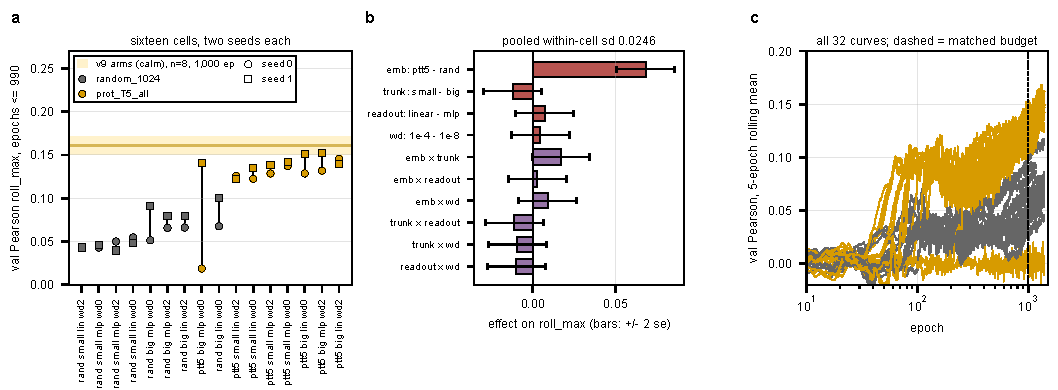
\includegraphics[width=\textwidth]{figures/v10_grid_factorial.pdf}
\caption[]{\textbf{The v10 grid at a matched budget.} \textbf{a}, every cell's two seeds at
epochs $\le 990$, sorted by cell mean and colored by embedding, against the eight
long-budget v9 arms at 1{,}000 epochs ($0.161 \pm 0.010$, \file{calm} embeddings, band is
one standard deviation across arms). \textbf{b}, main effects and two-way
interactions with $\pm 2$ standard errors from the pooled within-cell spread.
\textbf{c}, all 32 validation curves; the dashed line is the matched budget. Generated by
\file{v10_grid_factorial.py}.}
\label{fig:readouts-factorial}
\end{figure}

\pfstep{Embedding content is worth $0.07$, three times the replicate spread.} The ProtT5
cells average $0.129$ against $0.061$ for random vectors of the same width, and no cell of
one level overlaps any cell of the other (\cref{fig:readouts-factorial}a). The contrast was
built as a content test at matched width 1{,}024, so it says the content matters and says
nothing about \file{calm}, the incumbent's embedding, which is not a level of the grid. The
one healthy draw of the incumbent-with-ProtT5 cell scores $0.141$ against the incumbent's
$0.161 \pm 0.010$ at the same budget, one draw against eight, and that is not a resolved gap
in either direction.

\pfstep{Readout width and weight decay are measured nulls.} Both effects are under $0.008$
against a resolution of about $0.02$ at two standard errors. The trunk is a small effect in
favor of the deeper one, $-0.012$ over all runs and $-0.018$ once the stuck run is dropped,
and it is sharper under ProtT5 (the interaction). Of the four factors chosen to act on the
train-validation gap, one acts.

\pfstep{One run in 32 never learned.} Cell 1 seed 0 (\texttt{te8272kk}: ProtT5, $L{=}6$,
two-layer readout, weight decay $10^{-8}$) sits at $0.019$ at its best and $-0.007$ at
epoch 1{,}399 with \file{nmse} $1.010$, while its seed-1 twin is the grid's best single run
at $0.169$. That pair alone carries most of the pooled variance, which is why both readings
are given. Its cause is not measured.

\subsection{The mechanism round: per-gene readout $+0.03$, under the round's resolution
\secstatus{todo}}
\label{sec:readouts-mech}

All four array tasks of the round ended in the cgroup out-of-memory handler at host RSS
61~GB against a 60~GB request, after 3.5 to 4.6 days. In each task one of the two packed
runs was killed and the other finished its 8{,}500 epochs, so the matched budget is set by
the shortest survivor, epochs $\le 4{,}079$. The two seed-1 runs abandoned on cabbi at epoch
${\approx}1{,}595$ when that half moved to the A40 node are superseded, not replicates, and
are dropped.

\begin{table}[htbp]
\centering\small
%% SOURCE: results/mech_round_readout.json, roll_max_le_4079 and paired_contrasts["4079"]
\begin{tabular}{lrrrr}
\toprule
arm & seed 0 & seed 1 & paired difference vs \texttt{R\_ref} (s0 / s1) & mean \\
\midrule
\texttt{R\_ref}               & $0.188$ & $0.169$ & & \\
\texttt{R\_basis64}           & $0.175$ & $0.200$ & $-0.014$ / $+0.030$ & $+0.008$ \\
\texttt{R\_pergene}           & $0.189$ & $0.224$ & $+0.001$ / $+0.054$ & $+0.028$ \\
\texttt{R\_pergene\_basis64}  & $0.214$ & $0.199$ & $+0.026$ / $+0.029$ & $+0.027$ \\
\bottomrule
\end{tabular}
\caption[]{The mechanism round at epochs $\le 4{,}079$, paired within seed against the
in-round reference. Seed 0 ran on cabbi Ada cards, seed 1 on one A40 node, so GPU type is
a seed-level block. The eight long-budget v9 arms score $0.188 \pm 0.017$ at 4{,}000
epochs and both \texttt{R\_ref} draws fall inside that band.}
\label{tab:readouts-mech}
\end{table}

\begin{figure}[htbp]
\centering
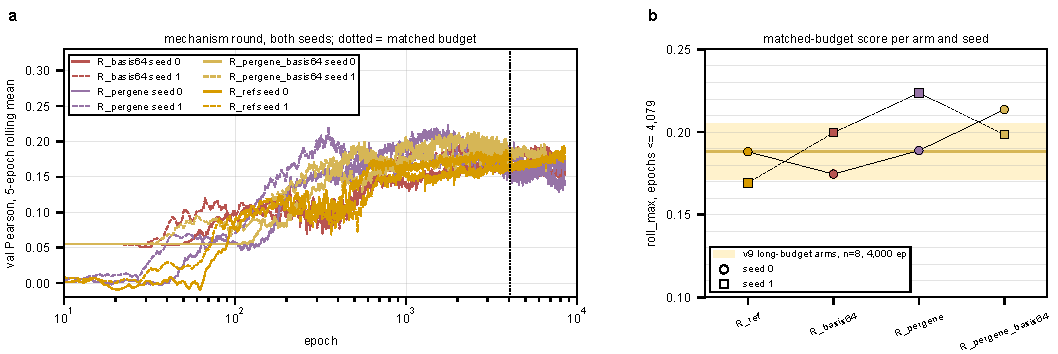
\includegraphics[width=\textwidth]{figures/mech_round_readout.pdf}
\caption[]{\textbf{The mechanism round.} \textbf{a}, validation Pearson of all eight runs
(solid seed 0, dashed seed 1); the dotted line is the matched budget. \textbf{b}, the
matched-budget score per arm and seed against the long-budget arm band at 4{,}000 epochs.
Generated by \file{mech_round_readout.py}.}
\label{fig:readouts-mech}
\end{figure}

\pfstep{The pair term alone is a null.} Its two paired differences disagree in sign and
average $+0.008$. The per-gene readout arms average $+0.027$, and the combined arm is
positive at both seeds, but the round was sized to resolve about $0.06$ at two pairs
(\cref{tab:findings-power}), so this is a direction and not a result. What every curve does
show is the dynamics: the per-gene arms reach their peak between epochs 1{,}200 and 2{,}600
and give part of it back (\texttt{R\_pergene} ends at $0.137$ and $0.170$ against peaks of
$0.189$ and $0.224$), while the reference and basis arms are flat or still rising at 8{,}500.
Whether the give-back is overfitting of the extra per-gene parameters is a hypothesis and
is not measured.

\pfstep{A tagging defect, found in the readout.} The arm script carried a wave-4b
\texttt{R\_ref} branch ahead of the wave-5 one; a shell \texttt{case} takes its first
match, so every reference run of this round is tagged \file{stage-wave4b}. The readout
selects by arm and config tag, and the shadowing branch is removed.

\subsection{The metric-aligned round at day two: collapse is the rule at batch 32
\secstatus{todo}}
\label{sec:readouts-pearson}

Three arms train on $1 - r$ directly, the mean per-feature Pearson over the genes hidden at
the current unmasking step (\file{pearson}), the same plus a masked squared error at unit
weight (\file{pearson_mse}), and the pure loss at batch 64 (\file{pearson_b64}), on IGB cabbi
from 2026-09-06. The two batch-32 arms run three seeds at two runs per card, the batch-64
arm two seeds solo. They were read at 1.9 of their 5 days, so every number here is partial
and the readout script records the epoch reached.

\begin{table}[htbp]
\centering\small
%% SOURCE: results/pearson_round_readout.json, read 2026-09-08 16:40 CT
\begin{tabular}{llrrrrr}
\toprule
arm & seed & epoch & \file{roll_max} @ epoch & last & on the floor from & spread ratio at end \\
\midrule
\file{pearson}     & 0 & 3{,}902 & $0.145$ @ 215   & $0.000$ & 584   & $0.000$ \\
\file{pearson}     & 1 & 3{,}886 & $0.133$ @ 151   & $0.000$ & 2{,}203 & $0.000$ \\
\file{pearson}     & 2 & 3{,}021 & $0.137$ @ 242   & $0.000$ & 680   & $0.000$ \\
\file{pearson_mse} & 0 & 3{,}899 & $0.137$ @ 138   & $0.000$ & 360   & -- \\
\file{pearson_mse} & 1 & 3{,}888 & $0.194$ @ 3{,}193 & $0.168$ & alive & $0.43$ \\
\file{pearson_mse} & 2 & 3{,}023 & $0.035$ @ 5     & $0.000$ & 14    & -- \\
\file{pearson_b64} & 0 & 6{,}051 & $0.194$ @ 1{,}926 & $0.163$ & alive & $0.80$ \\
\file{pearson_b64} & 1 & 6{,}049 & $0.186$ @ 2{,}419 & $0.138$ & alive & $0.73$ \\
\bottomrule
\end{tabular}
\caption[]{The metric-aligned round, partial. ``On the floor from'' is the first epoch after
which the 5-epoch rolling mean of the validation Pearson stays under $0.02$; the seed-1
\file{pearson} run is near zero from epoch ${\approx}250$ and flickers above the line until
2{,}203. The spread ratio is predicted over true standard deviation
(\file{pred_sd_ratio}). The eight long-budget v9 arms score $0.188 \pm 0.017$ at 4{,}000
epochs and $0.192 \pm 0.018$ at 6{,}000.}
\label{tab:readouts-pearson}
\end{table}

\begin{figure}[htbp]
\centering
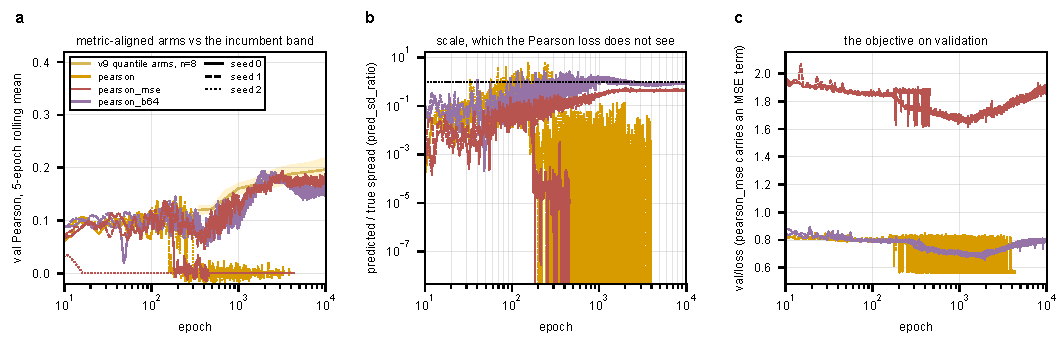
\includegraphics[width=\textwidth]{figures/pearson_round_readout.pdf}
\caption[]{\textbf{The metric-aligned round at day two.} \textbf{a}, validation Pearson of
all eight runs against the incumbent replicate band. \textbf{b}, predicted over true spread,
which the Pearson loss cannot see; a run whose outputs go constant falls off the bottom.
\textbf{c}, the objective on validation; \file{pearson_mse} carries the squared-error term
and sits on its own scale. Generated by \file{pearson_round_readout.py}.}
\label{fig:readouts-pearson}
\end{figure}

\pfstep{Five of six batch-32 runs are on the floor, and the loss does not see it.} The
three pure-Pearson runs peak between $0.13$ and $0.145$ at epochs 150 to 240 and then fall,
their predicted spread dropping from about $0.3$ to $10^{-7}$ over the same epochs
(\cref{fig:readouts-pearson}b): the network's output goes constant per gene. Their
validation loss holds near $0.56$ throughout, because the loss drops a constant column as
invalid and averages over the columns still varying, so it reads $1 - 0.44$ on a handful of
genes while the metric reads $0$ on all of them. The failure mode the design named is the
one that occurred, with the difference that the loss never reads its connected zero. The
squared-error anchor at unit weight did not prevent it: \file{pearson_mse} collapsed by
epoch 14 at one seed and 360 at another, and its surviving seed is alive at $0.194$ and
rising, inside the long-budget arm band.

\pfstep{The batch-64 runs survive and sit on the band, not above it.} Both are at 6{,}050
epochs with spread ratios of $0.73$ and $0.80$, \file{roll_max} $0.194$ and $0.186$
against the incumbent's $0.192 \pm 0.018$ at that budget, peaked near epochs 1{,}900 to
2{,}400 and drifting down since. Batch size and solo placement are confounded in that arm,
so why it survives is not measured; the in-batch correlation being taken over twice as many
strains is a hypothesis. Nothing in the round beats the quantile head at any budget read so
far, and the question it was launched to answer, whether the metric's late rise is
generalization gap or objective disagreement, is answerable only on the live runs after the
wall.

\subsection{Packed five-day runs die of host memory\secstatus{todo}}
\label{sec:readouts-oom}

Four of four packed tasks that ran past three and a half days ended \file{OUT_OF_MEMORY}
(\texttt{2369697} 0--1, \texttt{2371531} 2--3), at \file{MaxRSS} 61.4 and 61.1~GB. The
Pearson-round packed tasks read 21.3~GB at 1.9 days and the solo batch-64 tasks 17.2~GB.
Hypothesis (untested): resident memory grows roughly linearly through a run, in which case
the packed Pearson tasks reach the 60~GB line near day five, at the edge of their wall. What
grows is not identified; the \file{file_system} sharing strategy introduced in
\texttt{f1bfa95b} to stop the file-descriptor exhaustion is the obvious suspect and is
unverified. The memory of a running job cannot be raised, and the two rounds that finished
lost one run per task to it rather than the whole task.
